\documentclass[review,sigconf]{acmart}

\usepackage{graphicx}
\usepackage{listings}
\usepackage{multirow}
\usepackage{balance}
\usepackage{amsmath}
\usepackage{framed}
\usepackage{subfigure}

\newcommand{\todo}[1]{\textcolor{red}{TODO: #1}}

\begin{document}

\begin{titlepage}
    \begin{center}
        \vspace*{1cm}
            
        \Huge
        \textbf{Optical Music Recognition for LilyPond File Generation}
            
        \vspace{0.5cm}
        \LARGE
            
        \vspace{0.5cm}
            
        \textbf{Evan Matthews}

        \vspace{0.9cm}
		\textbf{Executive Summary}

		\vspace{0.5cm}
		This report explores the feasibility of Lilypond as a digital music format in the process of optical music recognition and translation for full scores.
		A simple Convolutional Recurrent Neural Network (CRNN) implementation was trained on Inventions by Johann Sebastian Bach, and test outputs of other Bach works were analyzed for generalization in the Lilypond format.
		Overall, \todo{results} 

		\begin{figure}
			\centering
			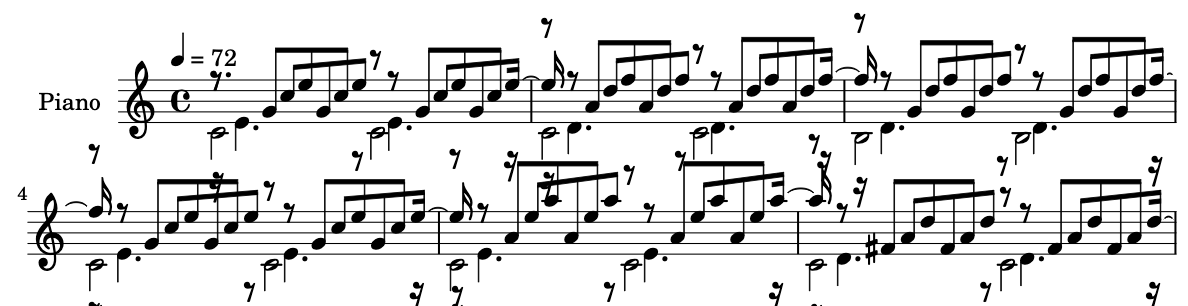
\includegraphics[width = .8\linewidth]{./figures/cover.png}
		\end{figure}

        \vfill
            
        \vspace{0.8cm}
            
        \Large
        Department of Computer Science\\
        University of Illinois Urbana-Champaign\\
        United States\\
        May 10th, 2024
            
    \end{center}
\end{titlepage}

\title[omr-lilypond-midi]{Optical Music Recognition for LilyPond File Generation}
\author{Evan Matthews}
% \email{evanmm3@illinois.edu}
% %\orcid{1234-5678-9012}
% \affiliation{%
% 	\institution{University of Illinois Urbana-Champaign}
% 	\country{}
% }

% \begin{abstract}
% \todo{Abstract}
% \end{abstract}

\maketitle

\section{Introduction}
\subsection{Initial Proposal}
\todo{Introduction citations}
\cite{andrea2021note}

In the world of music or audio transcription/arrangement, the complexity of sound and score data has allowed human performance to remain the current state-of-the-art. 
Several factors contribute to this circumstance: the number of potential audio and score file types, ambiguity on how performance qualities are notated, and overall inconsistencies between recordings and their respective scores. 
Machine learning models, in turn, have been a crucial step towards reducing these inconsistencies. 
Their ability to learn the nonlinearities and artistic qualities that otherwise plague audio computation have allowed for noteworthy advancements such as the WaveNet~\cite{oord2016wavenet}. 
The remaining issue in the process of sound generation is the amount of data available to train with. 
Worthwhile audio data remains difficult to collect due to its large size and potential copyright issues. 
In particular, trying to condition off another medium is incredibly difficult as current datasets lack the correlations necessary to streamline the audio transcription process. 
Datasets such as MAESTRO ~\cite{hawthorne2018enabling} are close to ideal results, but some intermediate steps are needed to learn correlations between audio files and musical scores.

With the following conditions in mind, I propose an Image-to-MIDI model to serve a few purposes. First, this model serves to convert image data to relative musical data to a high degree of accuracy. The process of converting MIDI to an image is trivial, but the opposite is a known Optical Music Recognition (OMR) problem in that the correlation is nonexistent. 
Second, a highly reliable model of this type is capable of serving as an intermediate step in future audio computation endeavors, as the nontrivial nature of OMR is a barrier for reliable model training between scores and other types of audio data. 
Finally, a conversion of this type allows for more flexible datasets because MIDI can be converted into a number of other audio file types.

\subsection{Known Limitations}

Given the vast complexity of western music notation and intricacies in notation/time alignment, the proposed model has a pessimistic approach. 
That is, given a small subset of musical data (\textit{among all notated music}) and some model, results can be expected to only match expected outputs through one or more of: pitch, rhythm, duration, and overall formatting.
Existing research in OMR supports these expectations. First, several digital notation systems exist for music, including: 

\begin{itemize}
	\item Standards like \textit{MusicXML}, \textit{Lilypond} and \textit{MIDI},
	\item Software-specific formats from \textit{Musescore}, \textit{Sibelius} and \textit{Finale},
	\item \textit{KERN} from the Humdrum tool-set ~\cite{contreras2023omrpian},
	\item Mayer, et al.'s \textit{Linearized MusicXML} ~\cite{mayer2024practical}, and
	\item Contreras, et al.'s untitled "end-to-end OMR" encoding language ~\cite{contreras2023omrcnn}.
\end{itemize} 

Each format provides benefits and drawbacks towards generalized OMR, but combined research efforts have yet to hone in on a particular format.
Second, current research continues to limit its effective musical scope: constant genre, time period composed, single vs. multi-line pieces, and single vs. multiple measures, to name a few.
These limitations are to be expected as a means of balancing experiment accuracy with the subset of musical notation to be recognized. 
However, no paper to date has intended to capture a high accuracy while completely generalizing the space of recognizable music.

Finally, the state-of-the-art for machine-learning-based OMR lies in the implementation of Convolutional Recurrent Neural Networks (CRNN). 
This model type is preferred over CNN for its ability to learn data as order-dependent sequences- a crucial philosophy in parsing and understanding musical scores in general. 
However, it should be noted that CNNs are still viable for their non-order-dependent musical problems, such as Nugroho and Zahra's work on individual note and duration recognition ~\cite{nugroho_zahra_2024}.

\subsection{Research Questions}

Despite low research expectations, I believe that a few questions can be posed and answered for the purpose of bounding requirements on a larger, all-encompassing Image-to-MIDI model:

\begin{itemize}
	\item [\textbf{RQ1}] What forms of recognition can be expected from a generalized CRNN implementation?
	\item [\textbf{RQ2}] How does Lilypond recognition compare against other standard and custom formats?
	\item [\textbf{RQ3}] What conflicts currently prevent state-of-the-art models from further generalization?
\end{itemize}

For \textbf{RQ1}, I aim to recover noticeable results regarding the CRNN model's ability to generalize sequences of data from scores.
Hence, whether or not order-dependent training can pick up on note, rhythm or duration sequences will be crucial to my final analysis.
Next, promising results from \textbf{RQ1} will be compared against existing research to answer \textbf{RQ2}. 
In particular, the generalized CRNN model's ability to render score data as Lilypond (.ly) files is compared against other notation systems to determine if a more complex Lilypond-based model would be successful.
Finally, for \textbf{RQ3}, the results of CRNN model training are criticized on what should be generalized or further implemented in order to reliably translate score images into Lilypond data.
This research question refers to all-encompassing limitations such as in \textbf{1.2} along with experiment-specific limitations.

\section{Background}
\subsection{Optical Music Recognition}
\todo{OMR background}

\begin{itemize}
	\item \textbf{Symbol Recognition:} a
	\item \textbf{Music Transcription:} b
\end{itemize}

\subsection{Lilypond}
Lilypond was chosen for dataset file representation as it maintains accurate translation between digital (MIDI) and visual (image) notation systems~\cite{lilypond}.
In particular, translation from Lilypond to MIDI is trivial, and Lilypond provides a more intuitive representation of musical information compared to raw bytes of MIDI data.
This notation language consists of multiple layers to separate score components:

\begin{itemize}
		\item \textbf{Document level:} components related to page layout and high-level musical details, (number of instruments/tracks, score engraving information).
		\item \textbf{Music level:} components related to low-level musical details, (notes, rhythms, durations, key/time signatures, tempo).
\end{itemize}

At the document level, aspects of a score that stay mostly or completely constant throughout a piece are indicated by specific, indent-sensitive keywords.
For example, the number of voices/instruments and respective number of staves are initialized with the $\backslash{Voice}$ and $\backslash{context}$ commands,
while high-level musical information is initialized by commands such as $\backslash{time}$ for time signature, $\backslash{key}$ for key signature, and $\backslash{tempo}$ for performance speed in beats per minute.  

At the music level, rhythmic musical symbols are notated according to their pitches and relative time duration.
pitches are all characters ${a, b, c, d, e, f, g, r}$, where $r$ is a "rest" meaning no pitch occurs.
To ascend or descend in pitch beyond a single musical "octave," the $'$ and $,$ characters are appended to indicate one or more octave ascendings or descendings, respectively.
Pitches are also proceeded by a rhythmic value representing its duration in time.
These values are typically powers of two, (but can technically be any positive floating-point value), and they dictate how long a pitch is played with respect to the piece's time signature.
For example, a score with time signature = 2/4 indicates that each measure has two beats, and each beat is the length of a quarter note (hard-coded in the denominator).
In this case, the line $"c4 \quad d4"$ would represent two quarter (4) notes or a single measure in the provided time signature.
Additionally, notes without defined durational values take on the previous note's duration in a line, so a series of equal-duration notes is represented by one durational value.
Finally, separations between measures are made with $"| \% n"$, marking the end of measure $n$.
Figure~\ref{fig:lilypond-example} compares the rendering of a single staff of music with its relative Lilypond notation.
\footnote{The time signature $C$ or "common-time" is another common way of writing 4/4.}

\begin{figure}
	\begin{subfigure}
		\centering
		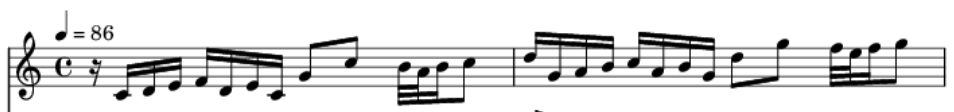
\includegraphics[width = .8\linewidth]{./figures/lilypond-snippet.png}
	\end{subfigure}
	~
	\begin{subfigure}
		\centering
		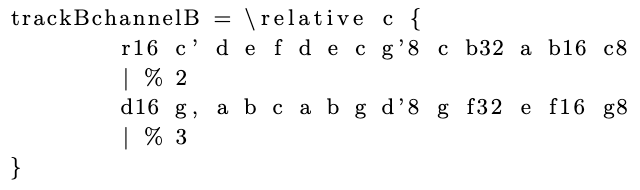
\includegraphics[width = .8\linewidth]{./figures/lilypond-code.png}
	\end{subfigure}
	\caption{Lilypond (.ly) code and rendering}
	\label{fig:lilypond-example}
\end{figure}

\section{Experiment}

\subsection{CRNN Model}
\todo{CRNN model}
The proposed Image-to-MIDI model is a smaller model referencing Shi, et al.'s pioneering work in the creation of CRNNs~\cite{shi2015endtoend}.
The model itself consists of multiple two-dimensional Convolutional/MaxPooling pairs for the purpose of extracting features from the intial score images.
Batch normalization layers are also applied to refine data recovered from the feature extraction.
Lastly, features are pushed through two bidirectional LSTM layers- the recurrent layers of the model- for data prediction with respect to "sequences" of the images.
In this case, sequences of the image data are the pixel columns of \todo{595?} $(595 \times H)$ images, where $H$ is the height of the image dependent on the overall "length" of the music.

\begin{figure}
	\centering
	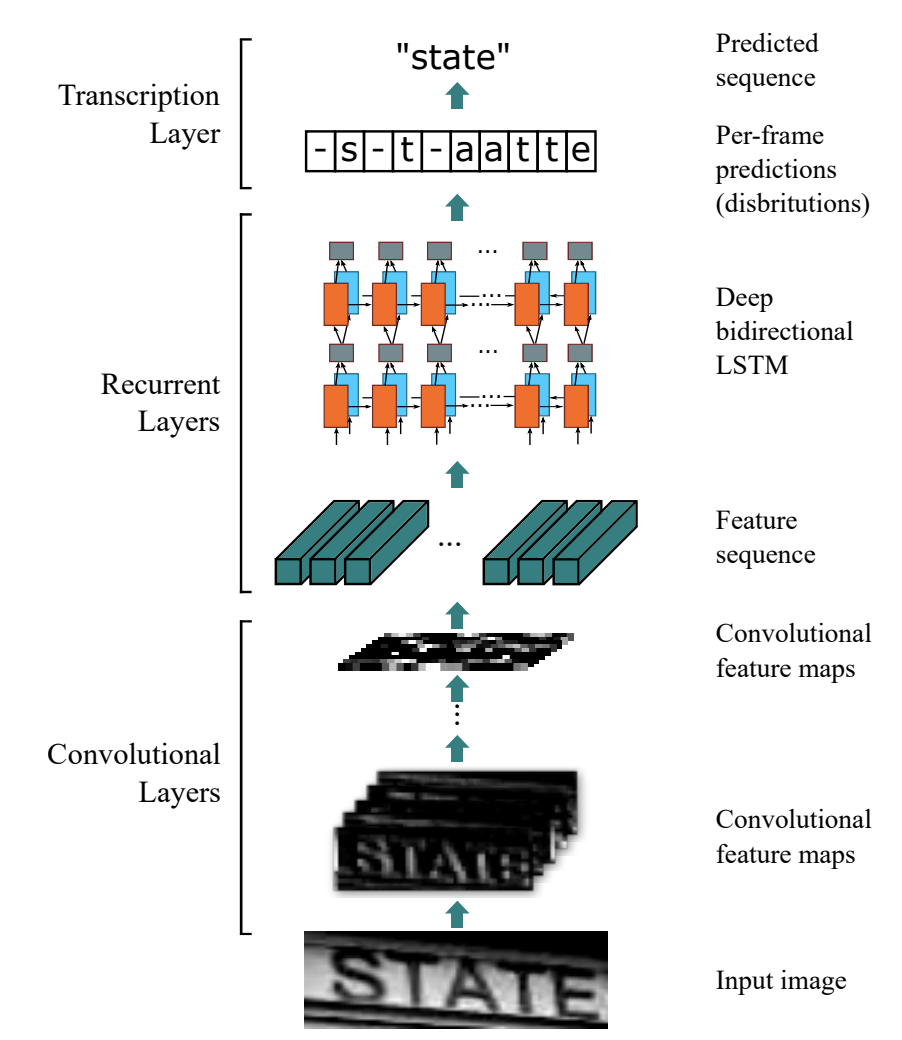
\includegraphics[width = .8\linewidth]{./figures/crnn_arch.png}
	\caption{General CRNN architecture, as modeled by Shi, et al. ~\cite{shi2015endtoend}}
	\label{fig:crnn-arch}
\end{figure}

\subsection{Data Specfications}
\todo{dataset specifics}
MIDI data used for this experiment has been narrowed down to strictly fifteen two-stave "inventions" by Johann Sebastian Bach ~\cite{bach_midi} to maintain rhythmic and compositional uniformity.
These works maintain relatively similar quantization schemes (rhythms and durations of notes), are short, and have several clear transcriptions for research, education, and entertainment purposes.

Testing was performed against a handful of arbitrary "preludes" and "fugues," also written by Bach. 
Limiting the training and testing sets, (especially in a way that limits the ability to calculate an overall accuracy), is purposefully done in the context of this experiment.
First, there are no expectations for relatively "accurate" recreations of score images in Lilypond. 
A proper training model would require extensive tokenization for all symbolic details that help to render a Lilypond file, which is outside of the scope of this research endeavor.
Rather, output is manually analyzed against its correlated image to determine what musical or notational qualities were generalized.
Second, a broader dataset would drastically complicate the CRNN model's ability to generalize key features of score images.
Focus on a single composer, musical time period, and music "type" (prelude, waltz, rondo, etc.) allows the model to more quickly generalize aspects of the subset of music, at the cost of potentially overfitting to the subset.


\begin{figure}
	\begin{subfigure}
		\centering
		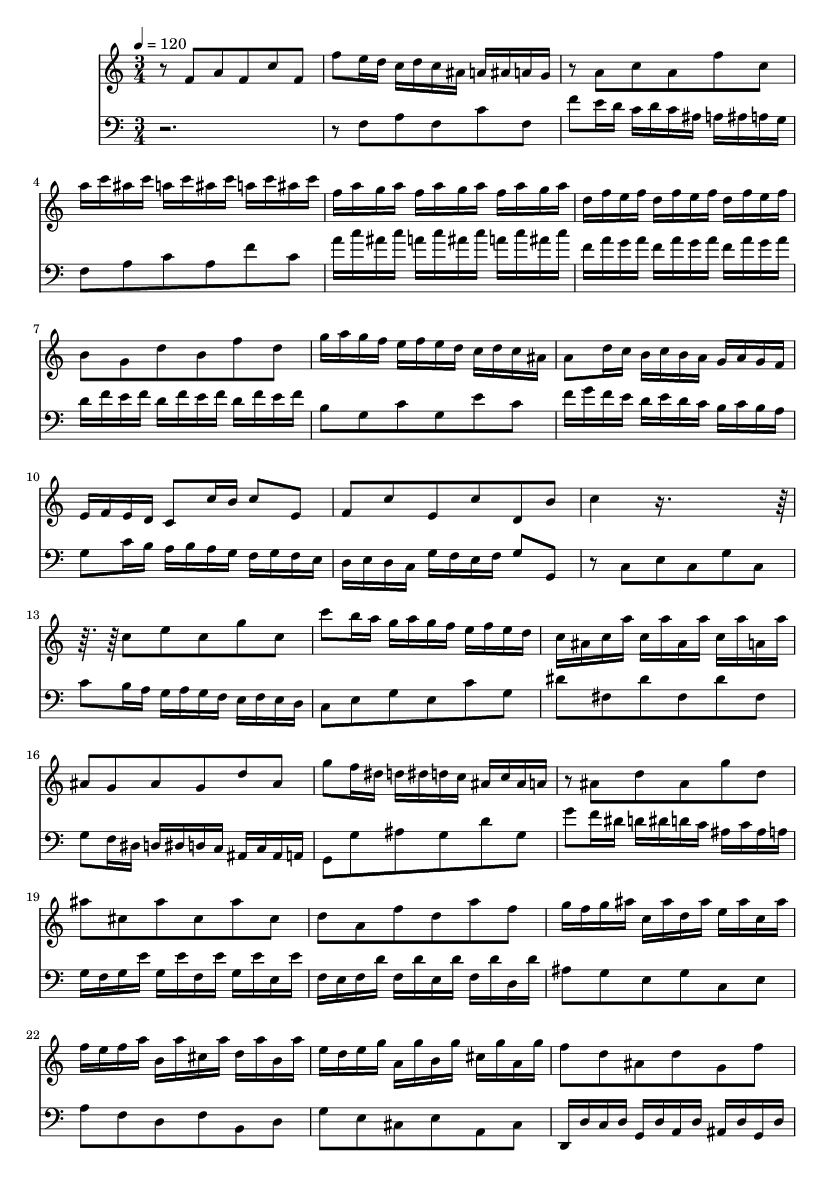
\includegraphics[width = .8\linewidth]{./figures/invent8.png}
	\end{subfigure}
	~
	\begin{subfigure}
		\centering
		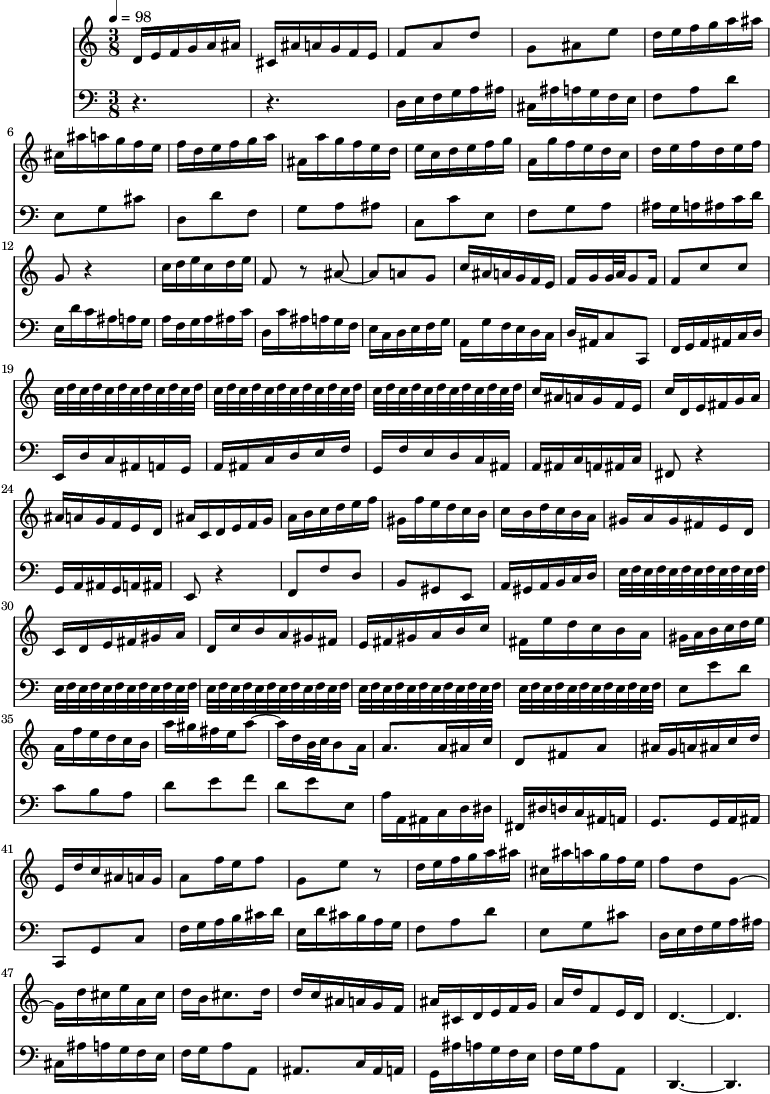
\includegraphics[width = .8\linewidth]{./figures/invent4.png}
	\end{subfigure}
	\caption{Excerpt of Invention No.4; cropped/prepared rendering of Invention No.8.}
	\label{fig:bach-example}
\end{figure}

\subsection{Quantization Rendering}
Similar to simple transformations performed on images, (rotations, coloring, scaling), output for sheet music determined by technical, but musical variables that don't affect the "performance" of the composition.
In particular, when score images are rendered from the Bach lilypond files, (trivially translated from the Bach MIDI Index~\cite{bach_midi}), there is a required "quantization" value which affects the rhythms and durations visually.
This quantization, designated $Q \in \mathbb{Z}$, represents what specific note duration counts as a "beat" within a given score. 
Figure ~\ref{fig:table-duration} lists the most common duration mappings that occur within this experiment.

\begin{figure}
	\centering
	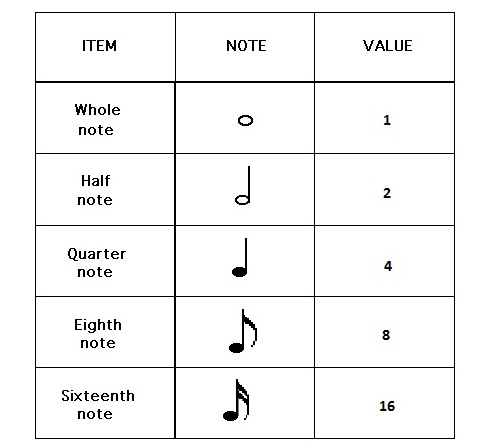
\includegraphics[width = .8\linewidth]{./figures/notevalues.jpeg}
	\caption{Table of common duration-integer mappings, from Francis Hamzagic ~\cite{hamzagic_2018}}
	\label{fig:table-duration}
\end{figure}

Drastic change of $Q$ results in score images that appear muddled or illegible despite conveying the same musical information, as shown in Figure ~\ref{fig:quantization}.
In order to prevent drastic shifts due to quantization, an optimal quantization $\hat Q$ is calculated with

\begin{figure}
	\centering
	\begin{subfigure}
		\centering
		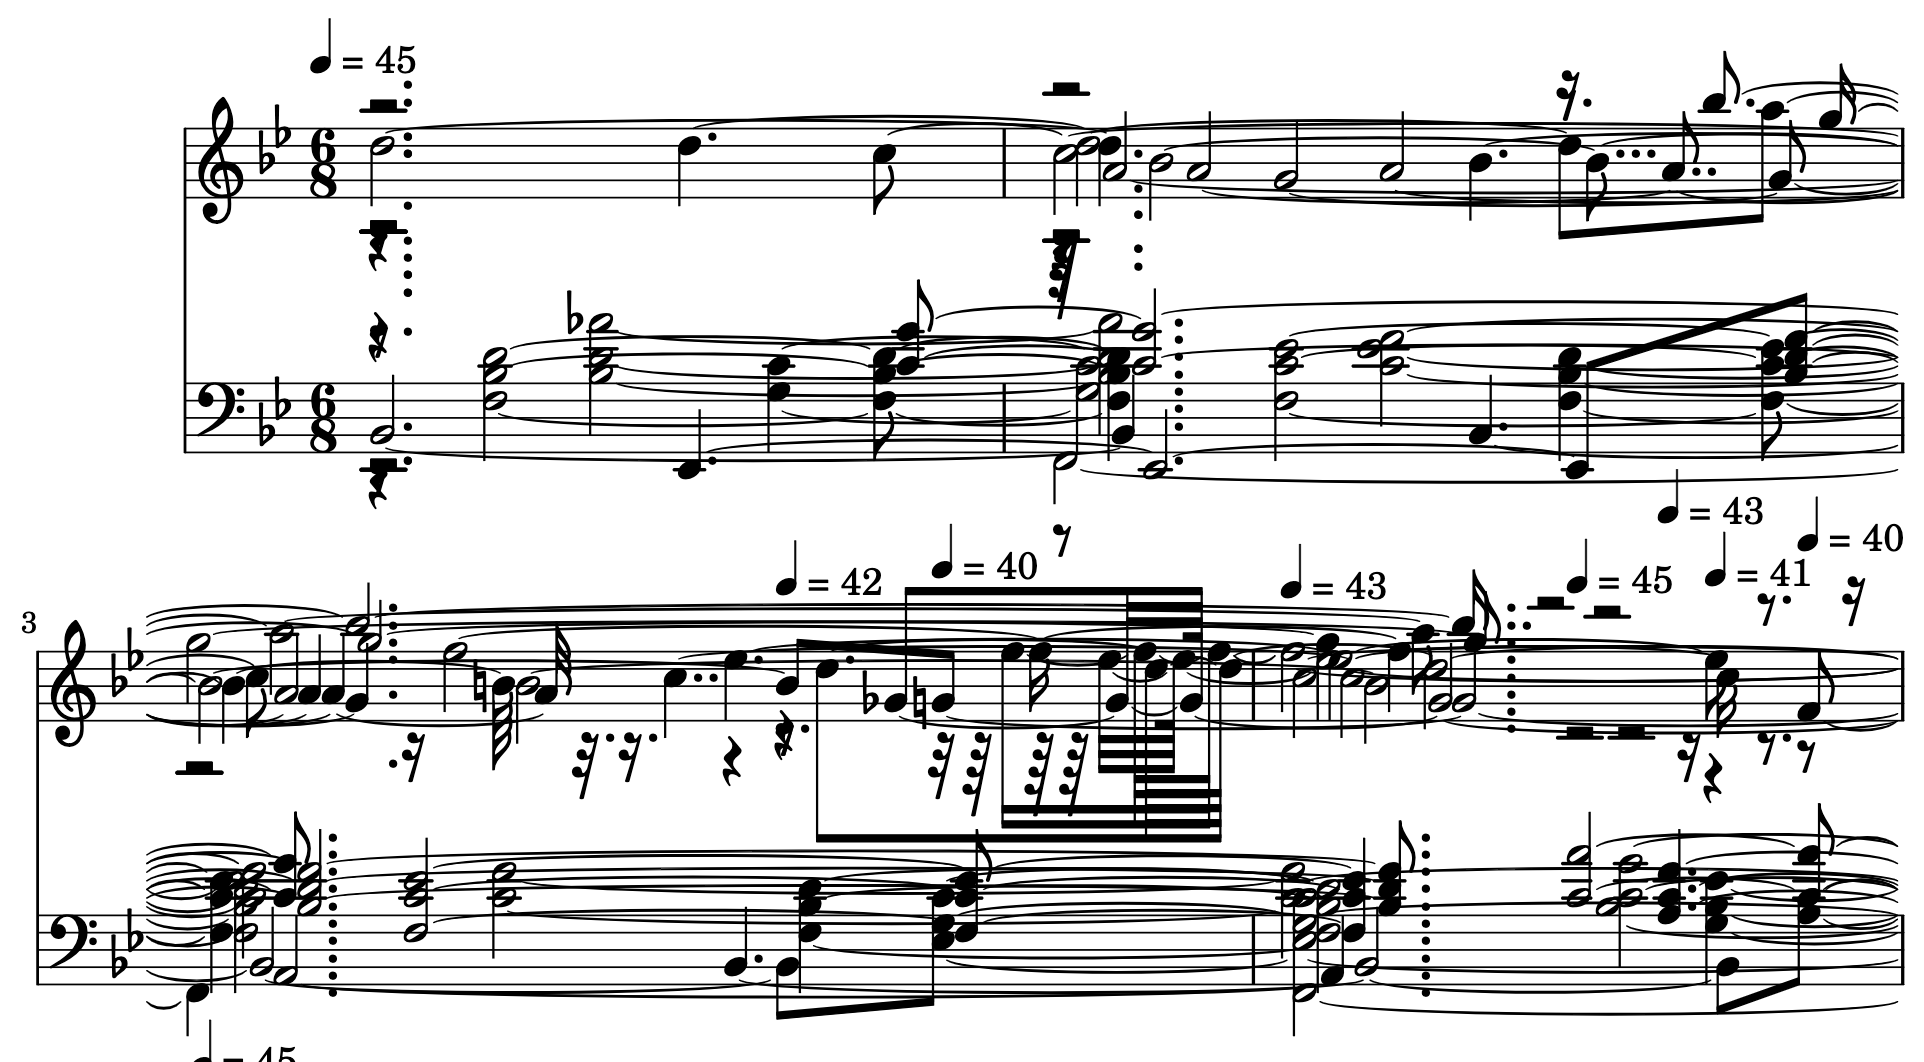
\includegraphics[width = .8\linewidth]{./figures/c1.png}
	\end{subfigure}
	~
	\begin{subfigure}
		\centering
		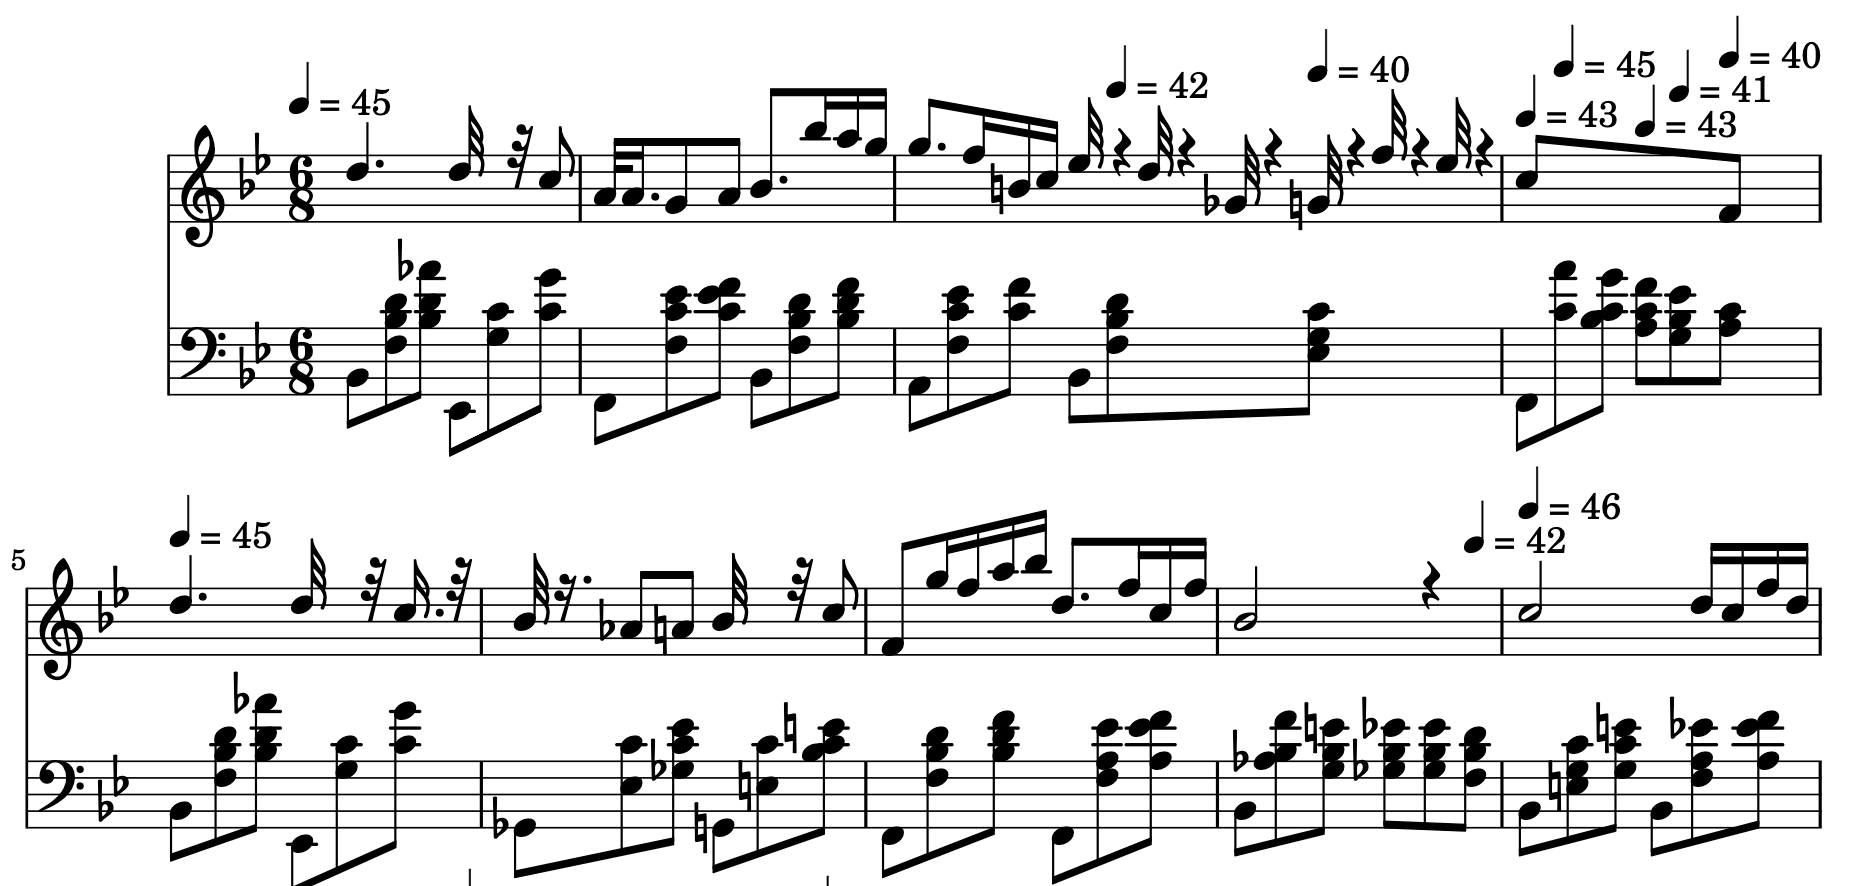
\includegraphics[width = .8\linewidth]{./figures/c32.png}
	\end{subfigure}
	\caption{Levels of Quantization $[2^0, 2^5]$ in Rendering}
	\label{fig:quantization}
\end{figure}

\begin{equation}
	\hat Q = \max_{t\in \text{MIDI events}} \frac{\tau * 10^{-6}}{t} * n * \text{floor}(d / 4)
\end{equation}

where $t$ is the number of seconds for a MIDI event to occur, $\tau$ is the provided MIDI tempo in beats per microsecond, and $(n, d)$ are the numerator and denominator, respectively, of the piece's time signature.
Additionally, possible $\hat Q$ are limited to powers of 2 greater than 0 in order to reduce complication from compound time signatures, (where beats are not represented by durations in Figure ~\ref{fig:table-duration}).


\section{Results}
\todo{results}

\section{Discussion}

The following section details my analysis with respect to previously discussed research questions.

\subsection{Model Generalization (RQ1)}

\subsection{Format Comparison (RQ2)}

\subsection{Model Criticism (RQ3)}

\section{Conclusions}
\todo{conclusions}

\bibliographystyle{ACM-Reference-Format}
\bibliography{references-cs444}

\end{document}